%iffalse
\let\negmedspace\undefined
\let\negthickspace\undefined
\documentclass[journal,12pt,onecolumn]{IEEEtran}
\usepackage[version=4]{mhchem}
\usepackage{chemformula} % for \ch if needed
\usepackage{chemfig}
\usepackage{chemmacros}
\chemsetup{modules = reactions} % Enables reaction arrows
\usepackage{graphicx}
\graphicspath{ {./images/} }

\usepackage{fancyhdr}
\usepackage{geometry}
\usepackage{lastpage}
\usepackage{cite}
\usepackage{amsmath,amssymb,amsfonts,amsthm}
\usepackage{enumitem,multicol}
\usepackage{algorithmic}
\usepackage{graphicx}
\usepackage{textcomp}
\usepackage{xcolor}
\usepackage{txfonts}
\usepackage{listings}
\usepackage{enumitem}
\usepackage{mathtools}
\usepackage{gensymb}
\usepackage{comment}
\usepackage[breaklinks=true]{hyperref}
\usepackage{tkz-euclide} 
\usepackage{listings}
\usepackage{gvv}                                        
%\def\inputGnumericTable{}                                 
\usepackage[latin1]{inputenc}                                
\usepackage{color}                                            
\usepackage{array}                                            
\usepackage{longtable}                                       
\usepackage{calc}                                             
\usepackage{multirow}                                         
\usepackage{hhline}                                           
\usepackage{ifthen}                                           
\usepackage{lscape}
\usepackage{tabularx}
\usepackage{array}
\usepackage{float}


\newtheorem{theorem}{Theorem}[section]
\newtheorem{problem}{Problem}
\newtheorem{proposition}{Proposition}[section]
\newtheorem{lemma}{Lemma}[section]
\newtheorem{corollary}[theorem]{Corollary}
\newtheorem{example}{Example}[section]
\newtheorem{definition}[problem]{Definition}
\newcommand{\BEQA}{\begin{eqnarray}}
\newcommand{\EEQA}{\end{eqnarray}}
\newcommand{\define}{\stackrel{\triangle}{=}}
\theoremstyle{remark}

\geometry{margin=1 in}

\pagestyle{fancy}
\fancyhead[L]{2014}
\fancyhead[C]{}
\fancyhead[R]{CE}
\fancyfoot[L]{CE}
\fancyfoot[C]{}
\fancyfoot[R]{\thepage/\pageref{LastPage}}

\setlength{\headheight}{14pt}
\setlength{\headsep}{5pt}
\setlength{\footskip}{20pt}


% Line thickness
\renewcommand{\headrulewidth}{0.4pt}
\renewcommand{\footrulewidth}{0.4pt}



% Marks the beginning of the document
\begin{document}



\title{
ASSIGNMENT 6: GATE 2014 \\
CE: CIVIL ENGINEERING}
\author{AI25BTECH11021 - Abhiram Reddy N}
\maketitle


\begin{enumerate} 

%----------------- Q1 ------------------
\item A student is required to demonstrate a high level of \textbf{comprehension} of the subject, especially in the social sciences.      \hfill{\brak{\textbf{GATE CE 2014}}} \\
The word closest in meaning to \textbf{comprehension} is

\begin{multicols}{4}
    
\begin{enumerate}
\item understanding
\item meaning
\item concentration
\item stability
\end{enumerate}
\end{multicols}


%----------------- Q2 ------------------
\item Choose the most appropriate word from the options given below to complete the following sentence.  \hfill{\brak{\textbf{GATE CE 2014}}}  \\
One of his biggest \_\_\_\_\_ was his ability to forgive.
\begin{multicols}{4}
    

\begin{enumerate}
\item vice
\item virtues
\item choices
\item strength
\end{enumerate}
\end{multicols}


%----------------- Q3 ------------------
\item Rajan was not happy that Sajan decided to do the project on his own. On observing his unhappiness, Sajan explained to Rajan that he preferred to work independently.    \hfill{\brak{\textbf{GATE CE 2014}}}  \\
Which one of the statements below is logically valid and can be inferred from the above sentences?
\begin{multicols}{4}
    

\begin{enumerate}
\item Rajan has decided to work only in a group.
\item Rajan and Sajan were formed into a group against their wishes.
\item Sajan had decided to give in to Rajan's request to work with him.
\item Rajan had believed that Sajan and he would be working together.
\end{enumerate}
\end{multicols}


%----------------- Q4 ------------------
\item If \(y = 5x^2 + 3\), then the tangent at \(x = 0, y = 3\) \hfill{\brak{\textbf{GATE CE 2014}}}
\begin{multicols}{4}
    

\begin{enumerate}
\item passes through \(x = 0, y = 0\)
\item has a slope of \(+1\)
\item is parallel to the x-axis
\item has a slope of \(-1\)
\end{enumerate}
\end{multicols}


%----------------- Q5 ------------------
\item A foundry has a fixed daily cost of Rs 50,000 wherever it operates and a variable cost of Rs 800Q, where Q is the daily production in tonnes. What is the cost of production in Rs per tonne for a daily production of 100 tonnes?  \hfill{\brak{\textbf{GATE CE 2014}}}

\begin{multicols}{4}

\begin{enumerate}
\item 800
\item 1000
\item 1200
\item 1300
\end{enumerate}
\end{multicols}

%----------------- Q6 ------------------
\item Find the odd one in the following group: ALRVX, EPVZB, ITZDF, OYEIK   \hfill{\brak{\textbf{GATE CE 2014}}}

\begin{multicols}{4}

\begin{enumerate}
\item ALRVX
\item EPVZB
\item ITZDF
\item OYEIK
\end{enumerate}
\end{multicols}


%----------------- Q7 ------------------
\item Anuj, Bhola, Chandan, Dilip, Eswar and Faisal live on different floors in a six-storeyed building (the ground floor is numbered 1, the floor above it 2, and so on). Anuj lives on an even-numbered floor. Bhola does not live on an odd numbered floor. Chandan does not live on any of the floors below Faisal's floor. Dilip does not live on floor number 2. Eswar does not live on a floor immediately above or immediately below Bhola. Faisal lives three floors above Dilip. Which of the following floor-person combinations is correct?  \hfill{\brak{\textbf{GATE CE 2014}}}

\begin{figure}[H]
\centering
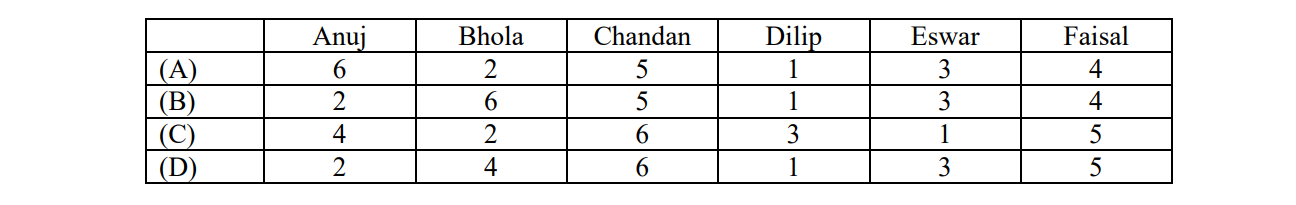
\includegraphics[width=\columnwidth]{figs/image1.png}
\caption{Floor-person combinations for Q7}
\label{fig:q7-floorplan}
\end{figure}



%----------------- Q8 ------------------
\item The smallest angle of a triangle is equal to two thirds of the smallest angle of a quadrilateral. The ratio between the angles of the quadrilateral is 3:4:5:6. The largest angle of the triangle is twice its smallest angle. What is the sum, in degrees, of the second largest angle of the triangle and the largest angle of the quadrilateral? \hfill{\brak{\textbf{GATE CE 2014}}}

%----------------- Q9 ------------------
\item One percent of the people of country X are taller than 6 ft. Two percent of the people of country Y are taller than 6 ft. There are thrice as many people in country X as in country Y. Taking both countries together, what is the percentage of people taller than 6 ft?  \hfill{\brak{\textbf{GATE CE 2014}}}

\begin{multicols}{4}
\begin{enumerate}
\item 3.0
\item 2.5
\item 1.5
\item 1.25
\end{enumerate}
\end{multicols}
%----------------- Q10 ------------------
\item The monthly rainfall chart based on 50 years of rainfall in Agra is shown in the following figure. Which of the following are true? (\textit{k percentile is the value such that k percent of the data fall below that value}) \hfill{\brak{\textbf{GATE CE 2014}}}
\begin{figure}[H]
\centering
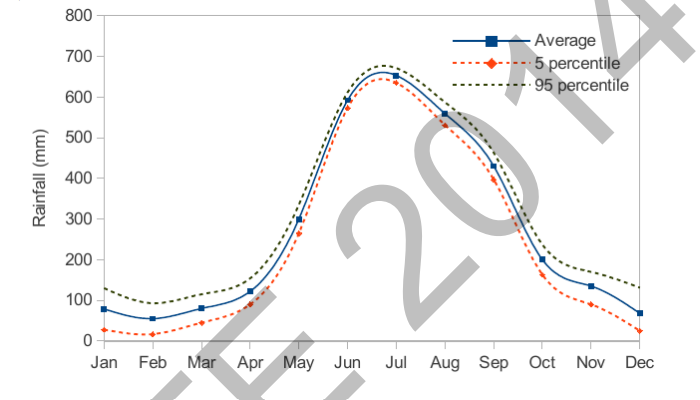
\includegraphics[width=0.75\textwidth]{figs/image2.png}
\caption{Monthly Rainfall in Agra}
\label{fig:monthly-rainfall-agra}
\end{figure}

\begin{enumerate}
\item On average, it rains more in July than in December
\item Every year, the amount of rainfall in August is more than that in January
\item July rainfall can be estimated with better confidence than February rainfall
\item In August, there is at least 500 mm of rainfall
\end{enumerate}

\begin{multicols}{4}

\begin{enumerate}
\item (i) and (ii)
\item (i) and (iii)
\item (ii) and (iii)
\item (iii) and (iv)
\end{enumerate}
\end{multicols}


\vspace{2 cm}

\begin{center}
    \textbf{END OF THE QUESTION PAPER}
\end{center}

\end{enumerate}

\newpage


\begin{enumerate}

%----------------- Q1 ------------------
\item 
\[
\lim_{x \to 0} \left(\frac{x + \sin x}{x}\right) \text{ equals to}
\]  \hfill{\brak{\textbf{GATE CE 2014}}}

\begin{multicols}{4}
\begin{enumerate}
\item $-\infty$
\item $0$
\item $1$
\item $\infty$
\end{enumerate}
\end{multicols}
%----------------- Q2 ------------------
\item Given the matrices 
\[
J = \myvec{3 & 2 & 1 \\ 2 & 4 & 2 \\ 1 & 2 & 6} \quad \text{and} \quad
K = \myvec{1 \\ 2 \\ -1},
\]
the product $K^T J K$ is \rule{3cm}{0.15mm}. \hfill{\brak{\textbf{GATE CE 2014}}}

%----------------- Q3 ------------------
\item The probability density function of evaporation $E$ on any day during a year in a watershed is given by \hfill{\brak{\textbf{GATE CE 2014}}}
\[
f(E) = \begin{cases}
\frac{1}{5} & 0 \leq E \leq 5 \text{ mm/day}\\
0 & \text{otherwise}
\end{cases}
\]
The probability that $E$ lies between 2 and 4 mm/day in a day in the watershed is (in decimal) \rule{3cm}{0.15mm}.

%----------------- Q4 ------------------
\item The sum of Eigen values of the matrix, $[M]$ is \hfill{\brak{\textbf{GATE CE 2014}}}
\[
[M] = \myvec{215 & 650 & 795 \\ 655 & 150 & 835 \\ 485 & 355 & 550}
\]

\begin{multicols}{4}

\begin{enumerate}
\item 915
\item 1355
\item 1640
\item 2180
\end{enumerate}
\end{multicols}

%----------------- Q5 ------------------
\item With reference to the conventional Cartesian $(x,y)$ coordinate system, the vertices of a triangle have the following coordinates: $(x_1,y_1) = (1,0)$; $(x_2,y_2) = (2,2)$; and $(x_3,y_3) = (4,3)$. The area of the triangle is equal to \hfill{\brak{\textbf{GATE CE 2014}}}


\begin{multicols}{4}

\begin{enumerate}
\item $\frac{3}{2}$
\item $\frac{3}{4}$
\item $\frac{4}{5}$
\item $\frac{5}{2}$
\end{enumerate}
\end{multicols}


%----------------- Q6 ------------------
\item Match the information given in Group - I with those in Group - II. \hfill{\brak{\textbf{GATE CE 2014}}} \\

\begin{multicols}{2}
Group - I

P \quad Factor to decrease ultimate strength to design strength

Q \quad Factor to increase working load to ultimate load for design

R \quad Statical method of ultimate load analysis

S \quad Kinematical mechanism method of ultimate load analysis
\columnbreak
Group - II

1 \quad Upper bound on ultimate load

2 \quad Lower bound on ultimate load

3 \quad Material partial safety factor

4 \quad Load factor
\end{multicols}

\begin{multicols}{2}
\begin{enumerate}
\item P - 1; Q - 2; R - 3; S - 4
\item P - 2; Q - 1; R - 4; S - 3
\item P - 3; Q - 4; R - 2; S - 1
\item P - 4; Q - 3; R - 2; S - 1
\end{enumerate}
\end{multicols}

%----------------- Q7 ------------------
\item The possible location of shear centre of the channel section, shown below, is \hfill{\brak{\textbf{GATE CE 2014}}}

\begin{figure}[H]
    \centering
    
\includegraphics[width=0.8\textwidth]{figs/image3.png}
    \caption{Shear Centre of Channel Section}
    \label{fig:shear-centre}
\end{figure}

\begin{multicols}{2}
\begin{enumerate}
\item P
\item Q
\item R
\item S
\end{enumerate}
\end{multicols}

%----------------- Q8 ------------------
\item The ultimate collapse load ($P$) in terms of plastic moment $M_p$ by kinematic approach for a propped cantilever of length $L$ with $P$ acting at its mid-span as shown in the figure, would be \hfill{\brak{\textbf{GATE CE 2014}}}

\begin{figure}[H]
    \centering
    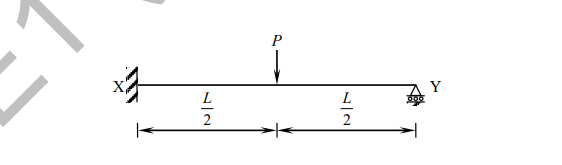
\includegraphics[width=0.8\textwidth]{figs/image4.png}
    \caption{Propped Cantilever Beam}
    \label{fig:propped-cantilever}
\end{figure}

\begin{multicols}{2}
\begin{enumerate}
\item $P = \frac{2M_p}{L}$
\item $P = \frac{4M_p}{L}$
\item $P = \frac{6M_p}{L}$
\item $P = \frac{8M_p}{L}$
\end{enumerate}
\end{multicols}

%----------------- Q9 ------------------
\item While designing, for a steel column of Fe250 grade, a base plate resting on a concrete pedestal of M20 grade, the bearing strength of concrete (in N/mm\textsuperscript{2}) in limit state method of design as per IS:456-2000 is \rule{3cm}{0.15mm}. \hfill{\brak{\textbf{GATE CE 2014}}}


%----------------- Q10 ------------------
\item A steel section is subjected to a combination of shear and bending actions. The applied shear force is $V$ and the shear capacity of the section is $V_s$. For such a section, high shear force (as per IS:800-2007) is defined as \hfill{\brak{\textbf{GATE CE 2014}}} \\

\begin{multicols}{2}
\begin{enumerate}
\item $V > 0.6V_s$
\item $V > 0.7V_s$
\item $V > 0.8V_s$
\item $V > 0.9V_s$
\end{enumerate}
\end{multicols}

%----------------- Q11 ------------------
\item The degree of static indeterminacy of a rigid jointed frame PQR supported as shown in the figure is \hfill{\brak{\textbf{GATE CE 2014}}}

\begin{figure}[H]
    \centering
    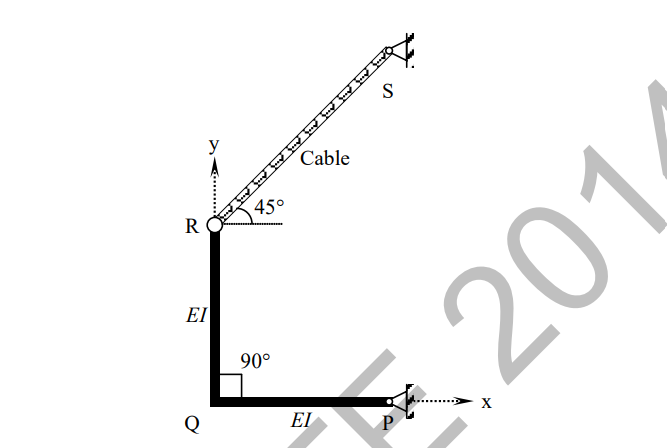
\includegraphics[width=0.8\textwidth]{figs/image5.png}
    \caption{Rigid Jointed Frame PQR}
    \label{fig:rigid-jointed-frame}
\end{figure}

\begin{multicols}{2}
\begin{enumerate}
\item zero
\item one
\item two
\item unstable
\end{enumerate}
\end{multicols}

%----------------- Q12 ------------------
\item In a beam of length $L$, four possible influence line diagrams for shear force at a section located at a distance of $\frac{L}{4}$ from the left end support (marked as P, Q, R and S) are shown below. The correct influence line diagram is \hfill{\brak{\textbf{GATE CE 2014}}}

\begin{figure}[H]
    \centering
    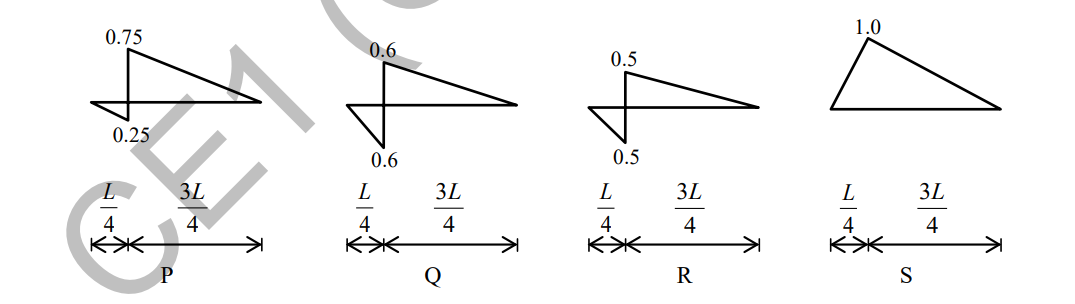
\includegraphics[width=0.8\textwidth]{figs/image6.png}
    \caption{Influence Line Diagrams for Shear Force}
    \label{fig:influence-line-diagrams}
\end{figure}

\begin{multicols}{2}
\begin{enumerate}
\item P
\item Q
\item R
\item S
\end{enumerate}
\end{multicols}

%----------------- Q13 ------------------
\item The degree of disturbance of the sample collected by the sampler is expressed by a term called the "area ratio". If the outer diameter and inner diameter of the sampler are $D_o$ and $D_i$ respectively, the area ratio is given by \hfill{\brak{\textbf{GATE CE 2014}}} \\

\begin{multicols}{2}
\begin{enumerate}
\item $\frac{D_o^2 - D_i^2}{D_i^2}$
\item $\frac{D_i^2 - D_o^2}{D_o^2}$
\item $\frac{D_o^2 - D_i^2}{D_o^2}$
\item $\frac{D_i^2 - D_o^2}{D_i^2}$
\end{enumerate}
\end{multicols}



%----------------- Q14 ------------------
\item For a saturated cohesive soil, a triaxial test yields the angle of internal friction ($\varphi$) as zero. The conducted test is \hfill{\brak{\textbf{GATE CE 2014}}}

\begin{multicols}{2}
\begin{enumerate}
\item Consolidated Drained (CD) test
\item Consolidated Undrained (CU) test
\item Unconfined Compression (UC) test
\item Unconsolidated Undrained (UU) test
\end{enumerate}
\end{multicols}

%----------------- Q15 ------------------
\item The action of negative skin friction on the pile is to \hfill{\brak{\textbf{GATE CE 2014}}}

\begin{multicols}{2}
\begin{enumerate}
\item increase the ultimate load on the pile
\item reduce the allowable load on the pile
\item maintain the working load on the pile
\item reduce the settlement of the pile
\end{enumerate}
\end{multicols}

%----------------- Q16 ------------------
\item A long slope is formed in a soil with shear strength parameters: $c' = 0$ and $\phi' = 34^\circ$. A firm stratum lies below the slope and it is assumed that the water table may occasionally rise to the surface, with seepage taking place parallel to the slope. Use $\gamma_{sat} = 18\, \text{kN/m}^3$ and $\gamma_w = 10\, \text{kN/m}^3$. The maximum slope angle (in degrees) to ensure a factor of safety of 1.5, assuming a potential failure surface parallel to the slope, would be \hfill{\brak{\textbf{GATE CE 2014}}}

\begin{multicols}{2}
\begin{enumerate}
\item 45.3
\item 44.7
\item 12.3
\item 11.3
\end{enumerate}
\end{multicols}

%----------------- Q17 ------------------
\item An incompressible homogeneous fluid is flowing steadily in a variable diameter pipe having the large and small diameters as 15 cm and 5 cm, respectively. If the velocity at a section at the 15 cm diameter portion of the pipe is 2.5 m/s, the velocity of the fluid (in m/s) at a section falling in 5 cm portion of the pipe is \hfill{\brak{\textbf{GATE CE 2014}}}

% No options or image given here.

%----------------- Q18 ------------------
\item A conventional flow duration curve is a plot between \hfill{\brak{\textbf{GATE CE 2014}}}


\begin{enumerate}
\item Flow and percentage time flow is exceeded
\item Duration of flooding and ground level elevation
\item Duration of water supply in a city and proportion of area receiving supply exceeding this duration
\item Flow rate and duration of time taken to empty a reservoir at that flow rate
\end{enumerate}


%----------------- Q19 ------------------
\item In reservoirs with an uncontrolled spillway, the peak of the plotted outflow hydrograph \hfill{\brak{\textbf{GATE CE 2014}}}


\begin{enumerate}
\item lies outside the plotted inflow hydrograph
\item lies on the recession limb of the plotted inflow hydrograph
\item lies on the peak of the inflow hydrograph
\item is higher than the peak of the plotted inflow hydrograph
\end{enumerate}



%----------------- Q20 ------------------
\item The dimension for kinematic viscosity is \hfill{\brak{\textbf{GATE CE 2014}}}

\begin{multicols}{4}
\begin{enumerate}
\item $\dfrac{L}{MT}$
\item $\dfrac{L}{T^{2}}$
\item $\dfrac{L^2}{T}$
\item $\dfrac{ML}{T}$
\end{enumerate}
\end{multicols}

%----------------- Q21 ------------------
\item Some of the nontoxic metals normally found in natural water are \hfill{\brak{\textbf{GATE CE 2014}}}

\begin{multicols}{2}
\begin{enumerate}
\item arsenic, lead and mercury
\item calcium, sodium and silver
\item cadmium, chromium and copper
\item iron, manganese and magnesium
\end{enumerate}
\end{multicols}

%----------------- Q22 ------------------
\item The amount of CO$_2$ generated (in kg) while completely oxidizing one kg of CH$_4$ to the end products is \hfill{\brak{\textbf{GATE CE 2014}}}

%----------------- Q23 ------------------
\item The minimum value of 15 minute peak hour factor on a section of a road is \hfill{\brak{\textbf{GATE CE 2014}}}

\begin{multicols}{4}
\begin{enumerate}
\item 0.10
\item 0.20
\item 0.25
\item 0.33
\end{enumerate}
\end{multicols}

%----------------- Q24 ------------------
\item The following statements are related to temperature stresses developed in concrete pavement slabs with free edges (without any restraint): \\

P. The temperature stresses will be zero during both day and night times if the pavement slab is considered weightless \\

Q. The temperature stresses will be compressive at the bottom of the slab during night time if the self-weight of the pavement slab is considered \\

R. The temperature stresses will be compressive at the bottom of the slab during day time if the self-weight of the pavement slab is considered \\

The TRUE statement(s) is(are) \hfill{\brak{\textbf{GATE CE 2014}}}

\begin{multicols}{4}
\begin{enumerate}
\item P only
\item Q only
\item P and Q only
\item P and R only
\end{enumerate}
\end{multicols}

%----------------- Q25 ------------------
\item The Reduced Levels (RLs) of the points P and Q are +49.600 m and +51.870 m respectively. Distance PQ is 20 m. The distance (in m from P) at which the +51.000 m contour cuts the line PQ is \hfill{\brak{\textbf{GATE CE 2014}}}

\begin{multicols}{4}
\begin{enumerate}
\item 15.00
\item 12.33
\item 3.52
\item 2.27
\end{enumerate}
\end{multicols}



\item If the following equation establishes equilibrium in slightly bent position, the mid-span deflection of a member shown in the figure is
\[
\frac{d^2 y}{dx^2} + \frac{P}{EI} y = 0
\]
If \(a\) is amplitude constant for \(y\), then \hfill{\brak{\textbf{GATE CE 2014}}}

\begin{figure}[H]
    \centering
    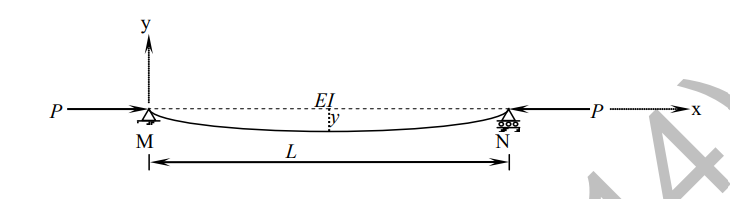
\includegraphics[width=0.7\textwidth]{figs/image7.png}
    \caption{Mid-span deflection of a member}
    \label{fig:q26}
\end{figure}

\begin{multicols}{4}
\begin{enumerate}
\item \( y = \frac{1}{P} \left(1 - a \cos \frac{2 \pi x}{L} \right) \)
\item \( y = \frac{1}{P} \left(a \sin \frac{2 \pi x}{L} \right) \)
\item \( y = a \sin \frac{n \pi x}{L} \)
\item \( y = a \cos \frac{n \pi x}{L} \)
\end{enumerate}
\end{multicols}

\item A box of weight 100 kN shown in the figure is to be lifted without swinging. If all forces are coplanar, the magnitude and direction \(\theta\) of the force \(F\) with respect to x-axis should be \hfill{\brak{\textbf{GATE CE 2014}}}

\begin{figure}[H]
    \centering
    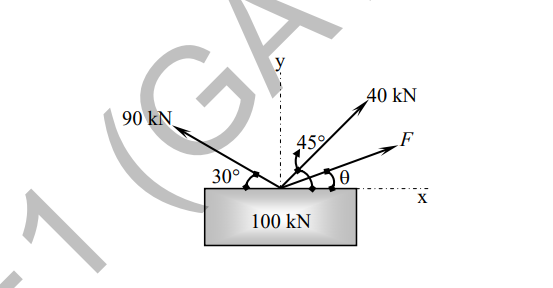
\includegraphics[width=0.6\textwidth]{figs/image8.png}
    \caption{Box being lifted}
    \label{fig:q27}
\end{figure}

\begin{multicols}{4}
\begin{enumerate}
\item \(F = 56.389 \text{ kN and } \theta = 28.28^\circ\)
\item \(F = -56.389 \text{ kN and } \theta = -28.28^\circ\)
\item \(F = 9.055 \text{ kN and } \theta = 1.414^\circ\)
\item \(F = -9.055 \text{ kN and } \theta = -1.414^\circ\)
\end{enumerate}
\end{multicols}

\item A particle moves along a curve whose parametric equations are:
\[
x = t^3 + 2t, \quad y = 3 e^{-2t}
\]
and
\[
z = 2 \sin(5t),
\]
where \(x, y\) and \(z\) show variations of the distance covered by the particle (in cm) with time \(t\) (in s). The magnitude of the acceleration of the particle (in cm/s\(^3\)) at \(t=0\) is \hfill{\brak{\textbf{GATE CE 2014}}}

\item A traffic office imposes on an average 5 number of penalties daily on traffic violators. Assume that the number of penalties on different days is independent and follows a Poisson distribution. The probability that there will be less than 4 penalties in a day is  \hfill{\brak{\textbf{GATE CE 2014}}}






%----------------- Q30 ------------------
\item Mathematical idealization of a crane has three bars with their vertices arranged as shown in the figure with a load of 80 kN hanging vertically. The coordinates of the vertices are given in parentheses. The force in the member $QR$, $F_{QR}$ will be \hfill{\brak{\textbf{GATE CE 2014}}}

\begin{figure}[H]
\centering
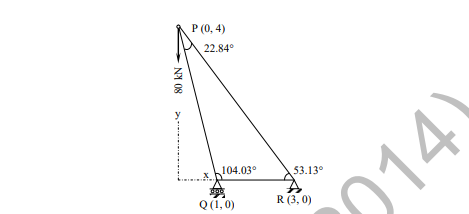
\includegraphics[width=0.7\linewidth]{figs/image9.png}
\caption{Crane truss configuration for Q30}
\label{fig:q30}
\end{figure}

\begin{multicols}{4}
\begin{enumerate}
\item 30 kN Compressive
\item 30 kN Tensile
\item 50 kN Compressive
\item 50 kN Tensile
\end{enumerate}
\end{multicols}

%----------------- Q31 ------------------
\item For the cantilever beam of span 3 m (shown below), a concentrated load of 20 kN applied at the free end causes a vertical displacement of 2 mm at a section located at a distance of 1 m from the fixed end. If a concentrated vertically downward load of 10 kN is applied at the section located at a distance of 1 m from the fixed end (with no other load on the beam), the maximum vertical displacement in the same beam (in mm) is \hfill{\brak{\textbf{GATE CE 2014}}}

\begin{figure}[H]
\centering

\includegraphics[width=0.7\linewidth]{figs/image10.png}
\caption{Cantilever beam setup for Q31}
\label{fig:q31}
\end{figure}

%----------------- Q32 ------------------
\item For the truss shown below, the member PQ is short by 3 mm. The magnitude of vertical displacement of joint R (in mm) is \hfill{\brak{\textbf{GATE CE 2014}}}

\begin{figure}[H]
\centering
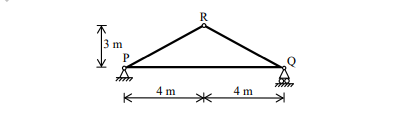
\includegraphics[width=0.7\linewidth]{figs/image11.png}
\caption{Truss deformation scenario for Q32}
\label{fig:q32}
\end{figure}






%----------------- Q33 ------------------
\item A rectangular beam of width $(b)$ 230 mm and effective depth $(d)$ 450 mm is reinforced with four bars of 12 mm diameter. The grade of concrete is M20 and grade of steel is Fe500. Given that for M20 grade of concrete the ultimate shear strength, $\tau_{cu} = 0.36$ N/mm$^2$ for steel percentage, $p = 0.25$, and $\tau_{cu} = 0.48$ N/mm$^2$ for $p = 0.50$. For a factored shear force of 45 kN, the diameter (in mm) of Fe500 steel two legged stirrups to be used at spacing of 375 mm, should be \hfill{\brak{\textbf{GATE CE 2014}}}

\begin{multicols}{4}
\begin{enumerate}
\item 8
\item 10
\item 12
\item 16
\end{enumerate}
\end{multicols}

%----------------- Q34 ------------------
\item The tension and shear force (both in kN) in each bolt of the joint, as shown below, respectively are \hfill{\brak{\textbf{GATE CE 2014}}}

\begin{figure}[H]
\centering
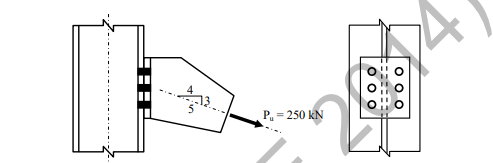
\includegraphics[width=0.7\linewidth]{figs/image12.png}
\caption{Bolt joint subjected to eccentric load (Q34)}
\label{fig:q34}
\end{figure}

\begin{multicols}{4}
\begin{enumerate}
\item 30.33 and 20.00
\item 30.33 and 25.00
\item 33.33 and 20.00
\item 33.33 and 25.00
\end{enumerate}
\end{multicols}

%----------------- Q35 ------------------
\item For a beam of cross-section, width = 230 mm and effective depth = 500 mm, the number of rebars of 12 mm diameter required to satisfy minimum tension reinforcement requirement specified by IS:456-2000 (assuming grade of steel reinforcement as Fe500) is \hfill{\brak{\textbf{GATE CE 2014}}}

%----------------- Q36 ------------------
\item In a reinforced concrete section, the stress at the extreme fibre in compression is 5.80 MPa. The depth of neutral axis in the section is 58 mm and the grade of concrete is M25. Assuming linear elastic behavior of the concrete, the effective curvature of the section (in per mm) is \hfill{\brak{\textbf{GATE CE 2014}}}

\begin{multicols}{4}
\begin{enumerate}
\item 2.0$\times 10^{-5}$
\item 3.0$\times 10^{-6}$
\item 4.0$\times 10^{-6}$
\item 5.0$\times 10^{-6}$
\end{enumerate}
\end{multicols}





%----------------- Q37 ------------------
\item Group I contains representative load-settlement curves for different modes of bearing capacity failures of sandy soil. Group II enlists the various failure characteristics. Match the load-settlement curves with the corresponding failure characteristics. \hfill{\brak{\textbf{GATE CE 2014}}}

\begin{figure}[H]
\centering
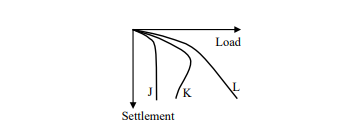
\includegraphics[width=0.4\linewidth]{figs/image13.png}
\caption{Load-settlement curves J, K, L for Q37}
\label{fig:q37}
\end{figure}

\textbf{Group I}
\begin{itemize}
\item P. Curve J
\item Q. Curve K
\item R. Curve L
\end{itemize}

\textbf{Group II}
\begin{enumerate}
\item No apparent heaving of soil around the footing
\item Rankine's passive zone develops imperfectly
\item Well defined slip surface extends to ground surface
\end{enumerate}

\begin{multicols}{4}
\begin{enumerate}
\item P - 1, Q - 3, R - 2
\item P - 3, Q - 2, R - 1
\item P - 3, Q - 1, R - 2
\item P - 1, Q - 2, R - 3
\end{enumerate}
\end{multicols}

%----------------- Q38 ------------------
\item A given cohesionless soil has $e_{max} = 0.85$ and $e_{min} = 0.50$. In the field, the soil is compacted to a mass density of 1800 kg/m$^3$ at a water content of 8\%. Take the mass density of water as 1000 kg/m$^3$ and $G_s$ as 2.7. The relative density (in \%) of the soil is \hfill{\brak{\textbf{GATE CE 2014}}}

\begin{multicols}{4}
\begin{enumerate}
\item 56.43
\item 60.25
\item 62.87
\item 65.71
\end{enumerate}
\end{multicols}

%----------------- Q39 ------------------
\item The following data are given for the laboratory sample. \hfill{\brak{\textbf{GATE CE 2014}}}

\[
\sigma_0' = 175 \text{ kPa}, \quad e_0 = 1.1 ; \qquad \sigma_1' = \sigma_0' + \Delta \sigma' = 300 \text{ kPa} ; \quad e = 0.9
\]

If thickness of the clay specimen is 25 mm, the value of coefficient of volume compressibility is $\rule{2cm}{0.15mm} \times 10^{-4}$ m$^2$/kN

\begin{multicols}{4}
\begin{enumerate}
\item 2.0
\item 3.0
\item 4.0
\item 5.0
\end{enumerate}
\end{multicols}






%----------------- Q40 ------------------
\item The flow net constructed for the dam is shown in the figure below. Taking the coefficient of permeability as $3.8 \times 10^{-4}$ m/s, the quantity of flow (in cm$^3$/s) under the dam per meter of dam is \hfill{\brak{\textbf{GATE CE 2014}}}

\begin{figure}[H]
\centering
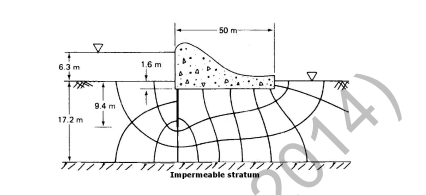
\includegraphics[width=0.92\linewidth]{figs/image14.png}
\caption{Flow net under dam (Q.40)}
\label{fig:q40}
\end{figure}

\begin{multicols}{4}
\begin{enumerate}
\item 64
\item 85
\item 40
\item 20
\end{enumerate}
\end{multicols}

%----------------- Q41 ------------------
\item A horizontal jet of water with its cross-sectional area of 0.0028 m$^2$ hits a fixed vertical plate with a velocity of 5 m/s. After impact the jet splits symmetrically in a plane parallel to the plane of the plate. The force of impact (in N) of the jet on the plate is \hfill{\brak{\textbf{GATE CE 2014}}}

\begin{multicols}{4}
\begin{enumerate}
\item 90
\item 80
\item 70
\item 60
\end{enumerate}
\end{multicols}

%----------------- Q42 ------------------
\item A venturimeter, having a diameter of 7.5 cm at the throat and 15 cm at the enlarged end, is installed in a horizontal pipeline of 15 cm diameter. The pipe carries an incompressible fluid at a steady rate of 30 liters per second. The difference of pressure head measured in terms of the moving fluid in between the enlarged and the throat of the venturimeter is observed to be 2.45 m. Taking the acceleration due to gravity as 9.81 m/s$^2$, the coefficient of discharge of the venturimeter (correct up to two places of decimal) is \hfill{\brak{\textbf{GATE CE 2014}}}

%----------------- Q43 ------------------
\item A rectangular channel having a bed slope of 0.0001, width 3.0 m and Manning's coefficient '$n$' = 0.015, carries a discharge of 1.0 m$^3$/s. Given that the normal depth of flow ranges between 0.76 m and 0.8 m. The minimum width of a throat (in m) that is possible at a given section, while ensuring that the prevailing normal depth is not exceeded along the reach upstream of the contraction, is approximately equal to (assume negligible losses) \hfill{\brak{\textbf{GATE CE 2014}}}

\begin{multicols}{4}
\begin{enumerate}
\item 0.64
\item 0.84
\item 1.04
\item 1.24
\end{enumerate}
\end{multicols}




%----------------- Q44 ------------------
\item Three rigid buckets, shown as in the figures (1), (2) and (3), are of identical heights and base areas. Further, assume that each of these buckets have negligible mass and are full of water. The weights of water in these buckets are denoted as $W_1$, $W_2$ and $W_3$ respectively. Also, let the force of water on the base of the bucket be denoted as $F_1$, $F_2$ and $F_3$ respectively. The option giving an accurate description of the system physics is \hfill{\brak{\textbf{GATE CE 2014}}}

\begin{figure}[H]
\centering
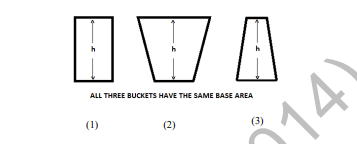
\includegraphics[width=0.55\linewidth]{figs/image15.png}
\caption{Three bucket shapes with identical heights and base areas (Q.44)}
\label{fig:q44}
\end{figure}

\begin{multicols}{4}
\begin{enumerate}
\item $W_2 = W_1 = W_3$ and $F_2 > F_1 > F_3$
\item $W_2 > W_1 > W_3$ and $F_2 > F_1 > F_3$
\item $W_2 = W_1 = W_3$ and $F_1 = F_2 = F_3$
\item $W_2 > W_1 > W_3$ and $F_1 = F_2 = F_3$
\end{enumerate}
\end{multicols}

%----------------- Q45 ------------------
\item An incompressible fluid is flowing at a steady rate in a horizontal pipe. From a section, the pipe divides into two horizontal parallel pipes of diameters $d_1$ and $d_2$ (where $d_1 = 4d_2$) that run for a distance of $L$ each and then again join back to a pipe of the original size. For both the parallel pipes, assume the head loss due to friction only and the Darcy-Weisbach friction factor to be the same. The velocity ratio between the bigger and the smaller branched pipes is \hfill{\brak{\textbf{GATE CE 2014}}}

%----------------- Q46 ------------------
\item 16 MLD of water is flowing through a 2.5 km long pipe of diameter 45 cm. The chlorine at the rate of 32 kg/d is applied at the entry of this pipe so that disinfected water is obtained at the exit. There is a proposal to increase the flow through this pipe to 22 MLD from 16 MLD. Assume the dilution coefficient, $\eta = 1$. The minimum amount of chlorine (in kg per day) to be applied to achieve the same degree of disinfection for the enhanced flow is \hfill{\brak{\textbf{GATE CE 2014}}}

\begin{multicols}{4}
\begin{enumerate}
\item 60.50
\item 44.00
\item 38.00
\item 23.27
\end{enumerate}
\end{multicols}

%----------------- Q47 ------------------
\item The potable water is prepared from turbid surface water by adopting the following treatment sequence. \hfill{\brak{\textbf{GATE CE 2014}}}

\begin{multicols}{2}
\begin{enumerate}
\item Turbid surface water $\rightarrow$ Coagulation $\rightarrow$ Flocculation $\rightarrow$ Sedimentation $\rightarrow$ Filtration $\rightarrow$ Disinfection $\rightarrow$ Storage \& Supply
\item Turbid surface water $\rightarrow$ Disinfection $\rightarrow$ Flocculation $\rightarrow$ Sedimentation $\rightarrow$ Filtration $\rightarrow$ Coagulation $\rightarrow$ Storage \& Supply
\item Turbid surface water $\rightarrow$ Filtration $\rightarrow$ Sedimentation $\rightarrow$ Disinfection $\rightarrow$ Flocculation $\rightarrow$ Coagulation $\rightarrow$ Storage \& Supply
\item Turbid surface water $\rightarrow$ Sedimentation $\rightarrow$ Filtration $\rightarrow$ Coagulation $\rightarrow$ Disinfection $\rightarrow$ Filtration $\rightarrow$ Storage \& Supply
\end{enumerate}
\end{multicols}






%----------------- Q48 ------------------
\item For a sample of water with the ionic composition shown in the figure below, the carbonate and non-carbonate hardness concentrations (in mg/l as CaCO$_3$), respectively are: \hfill{\brak{\textbf{GATE CE 2014}}}

\begin{figure}[H]
\centering
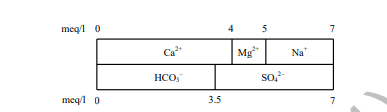
\includegraphics[width=0.6\linewidth]{figs/image16.png}
\caption{Ionic composition of water for hardness determination (Q.48)}
\label{fig:q48}
\end{figure}

\begin{multicols}{4}
\begin{enumerate}
\item 200 and 50
\item 175 and 75
\item 75 and 175
\item 50 and 200
\end{enumerate}
\end{multicols}

%----------------- Q49 ------------------
\item A straight 100 m long raw water gravity main is to carry water from an intake structure to the jack well of a water treatment plant. The required flow through this water main is 0.21 m$^3$/s. Allowable velocity through the main is 0.75 m/s. Assume $f = 0.01$, $g = 9.81$ m/s$^2$. The minimum gradient (in cm/100 m length) to be given to this gravity main so that the required amount of water flows without any difficulty is \hfill{\brak{\textbf{GATE CE 2014}}}

%----------------- Q50 ------------------
\item A traffic survey conducted on a road yields an average daily traffic count of 5000 vehicles. The axle load distribution on the same road is given in the following table: \hfill{\brak{\textbf{GATE CE 2014}}}

\begin{figure}[H]
\centering
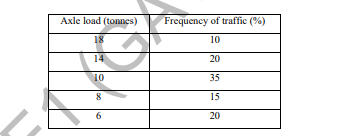
\includegraphics[width=0.7\linewidth]{figs/image17.png}
\caption{Axle load distribution table for MSA calculation (Q.50)}
\label{fig:q50}
\end{figure}

The design period of the road is 15 years, the yearly traffic growth rate is 7.5\% and the load safety factor (LSF) is 1.3. If the vehicle damage factor (VDF) is calculated from the above data, the design traffic (in million standard axle load, MSA) is

%----------------- Q51 ------------------
\item The perception-reaction time for a vehicle travelling at 90 km/h, given the coefficient of longitudinal friction of 0.35 and the stopping sight distance of 170 m (assume $g = 9.81$ m/s$^2$), is \hfill{\brak{\textbf{GATE CE 2014}}}

%----------------- Q52 ------------------
\item The speed-density ($u$-$k$) relationship on a single lane road with unidirectional flow is $u = 70 - 0.7k$, where $u$ is in km/hr and $k$ is in veh/km. The capacity of the road (in veh/hr) is \hfill{\brak{\textbf{GATE CE 2014}}}




%----------------- Q53 ------------------
\item An isolated three-phase traffic signal is designed by Webster's method. The critical flow ratios for three phases are 0.20, 0.30, and 0.25 respectively, and lost time per phase is 4 seconds. The optimum cycle length (in seconds) is \hfill{\brak{\textbf{GATE CE 2014}}}

\begin{multicols}{4}
\begin{enumerate}
\item 90
\item 95
\item 100
\item 105
\end{enumerate}
\end{multicols}

%----------------- Q54 ------------------
\item A levelling is carried out to establish the Reduced Levels (RL) of point R with respect to the Bench Mark (BM) at P. The staff readings taken are given below. \hfill{\brak{\textbf{GATE CE 2014}}}

\begin{figure}[H]
\centering
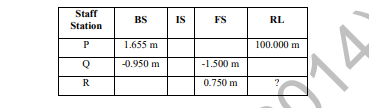
\includegraphics[width=0.7\linewidth]{figs/image18.png}
\caption{Staff readings and RL data for levelling (Q.54)}
\label{fig:q54}
\end{figure}

If RL of P is +100.000 m, then RL (in m) of R is

\begin{multicols}{4}
\begin{enumerate}
\item 103.355
\item 103.155
\item 101.455
\item 100.355
\end{enumerate}
\end{multicols}

%----------------- Q55 ------------------
\item Group I lists tool/instrument while Group II lists the method of surveying. Match the tool/instrument with the corresponding method of surveying. \hfill{\brak{\textbf{GATE CE 2014}}}

\textbf{Group I}
\begin{itemize}
\item[P.] Alidade
\item[Q.] Arrow
\item[R.] Bubble tube
\item[S.] Stadia hair
\end{itemize}

\textbf{Group II}
\begin{itemize}
\item[1.] Chain surveying
\item[2.] Levelling
\item[3.] Plane table surveying
\item[4.] Theodolite surveying
\end{itemize}

\begin{multicols}{4}
\begin{enumerate}
\item P - 3; Q - 2; R - 1; S - 4
\item P - 2; Q - 4; R - 3; S - 1
\item P - 1; Q - 2; R - 4; S - 3
\item P - 3; Q - 1; R - 2; S - 4
\end{enumerate}
\end{multicols}



\end{enumerate}
\vspace{3 cm}
\begin{center}
    \textbf{END OF THE QUESTION PAPER}
\end{center}







\end{document}